\def\QRCODE{MASTER_mispa_TUT.IMG.shape_from_focus_matlabqrcode.png}
\def\QRPAGE{http://www.iptutorials.science/tree/master/MASTER_mispa/TUT.IMG.shape_from_focus/matlab}
\mcorrectionsection{Matlab correction}

\subsection{Main function}
This function is used as the main function to perform shape-from-focus reconstruction. The parameter \minline{method} is the name of the function. Notice that tha variable \minline{stack} is of type \minline{double} to handle the cornea stack (which is a 16 bits image).

\begin{matlab}
function [Z, T]=SFF(file, N, method)
% Shape From Focus by SML method
% Z: heights/altitudes (indices)
% T: texture
%
% file: filename (tif stack-file)
% N: parameter of 'method' function
% method: method to use (SML, variance, etc.)
info = imfinfo(file);
num_images = numel(info);

% create stack into memory
stackF=zeros(info(1).Height, info(1).Width, num_images);

% load stack
stack =double(stackF);
for k = 1:num_images
    stack(:,:,k)=imread(file, k);
    % ... compute SML
    stackF(:,:,k) = feval(method, double(stack(:,:,k)), N);
end

% search for maximum of function
[~, Z] = max(stackF, [], 3);
Z = uint8(Z);
T = double(zeros(size(stack,1), size(stack,2)));
for i=1:size(T, 1)
    for j=1:size(T,2)
        T(i,j) = stack(i,j,Z(i,j));
    end
end

figure();
subplot(1,2,1); imshow(Z,[]); title('altitudes');
subplot(1,2,2); imshow(T,[]); title('textures');
end
\end{matlab}


\subsection{Sum of Modified Laplacian}
Results are illustrated in Fig.\ref{fig:sff:matlab:sml}.

\begin{matlab}
% main function
function SML=modifiedLaplacian(A, N)
     h1 = [0 0 0; -1 2 -1; 0 0 0];
     h2 = h1';
     ML = abs(conv2(A, h1, 'same')) + abs(conv2(A, h2, 'same'));
        
     h = ones(N);
     SML = conv2(ML, h, 'same');
end
\end{matlab}

\begin{figure}[htbp]
 \centering
 \subfloat[Texture.]{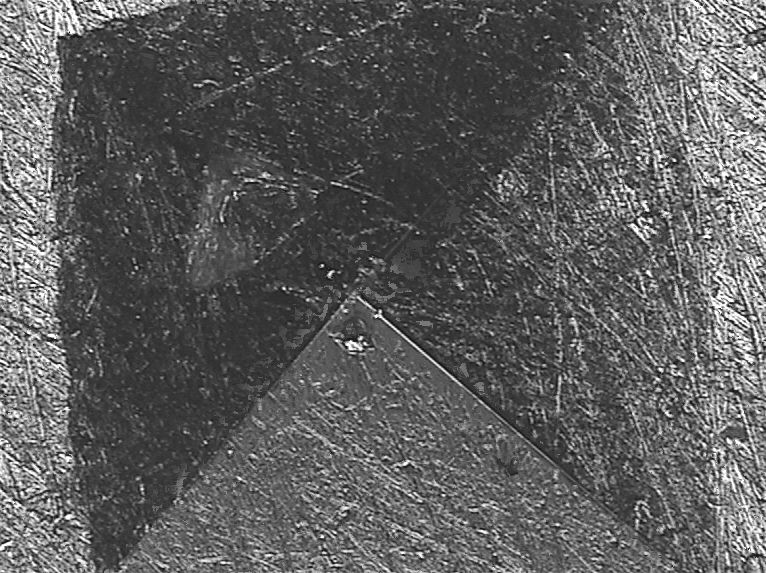
\includegraphics[width=.4\linewidth]{texture_SML_vickers.png}}\hfill
 \subfloat[Altitudes.]{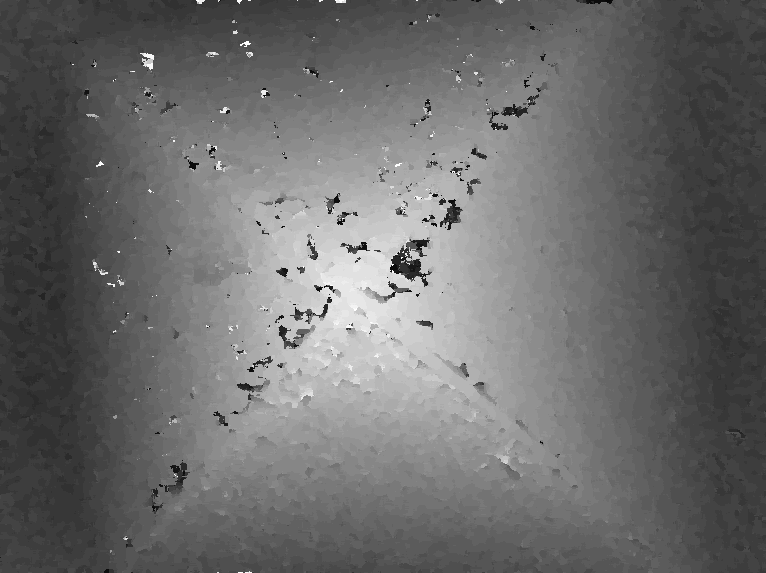
\includegraphics[width=.4\linewidth]{altitude_SML_vickers.png}}

 \subfloat[Texture.]{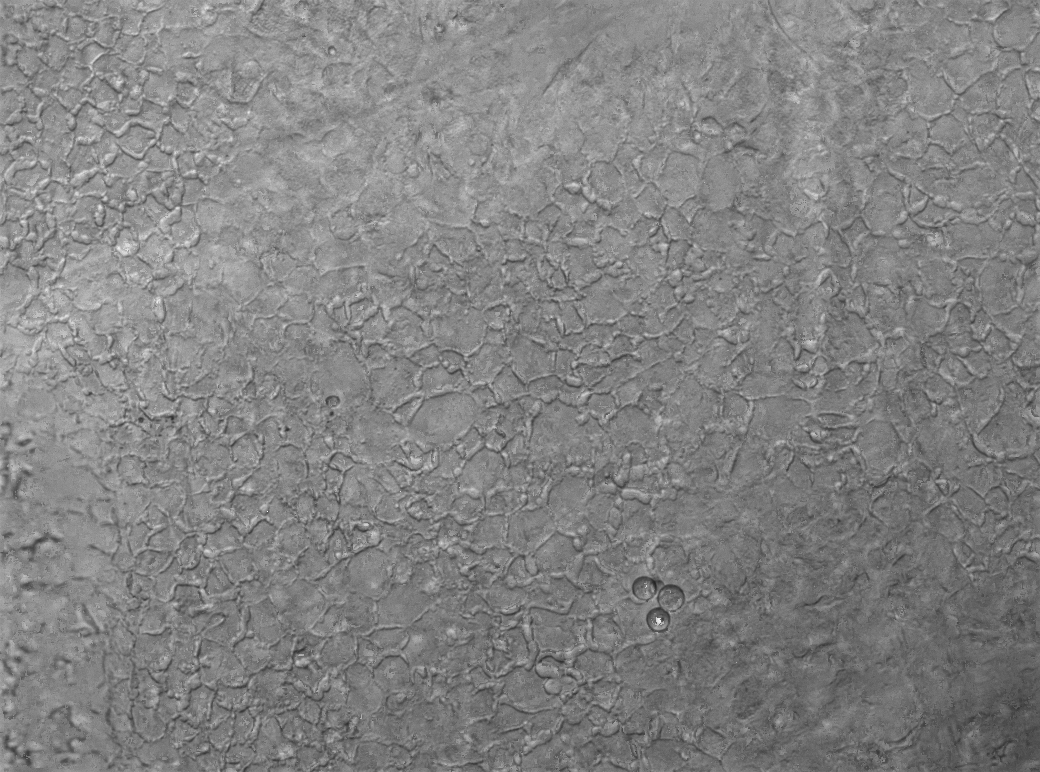
\includegraphics[width=.4\linewidth]{texture_SML_cornee.png}}\hfill
 \subfloat[Altitudes.]{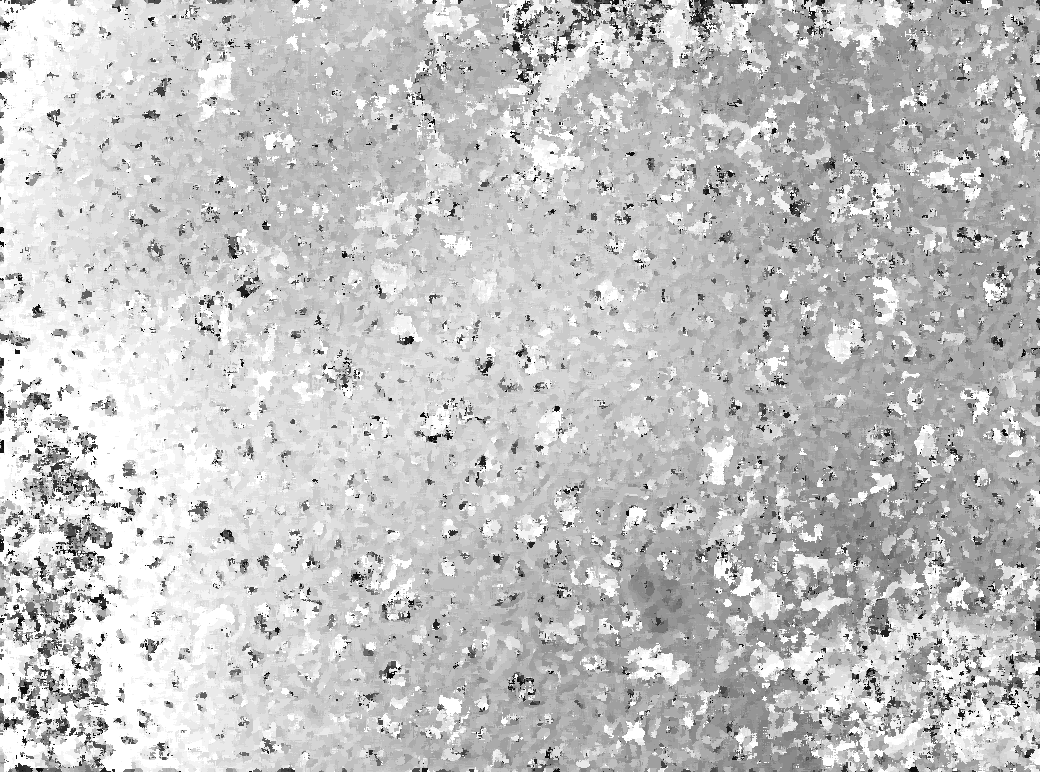
\includegraphics[width=.4\linewidth]{altitude_SML_cornee.png}}
 
 \caption{Texture and altitude reconstruction with the SML method.}
 \label{fig:sff:matlab:sml}
 
\end{figure}


\subsection{Variance}
The focus measure based on the variance i a really simple method that works in most cases, see Fig.\ref{fig:sff:matlab:variance}.

\begin{figure}[htbp]
 \centering
 \subfloat[Texture.]{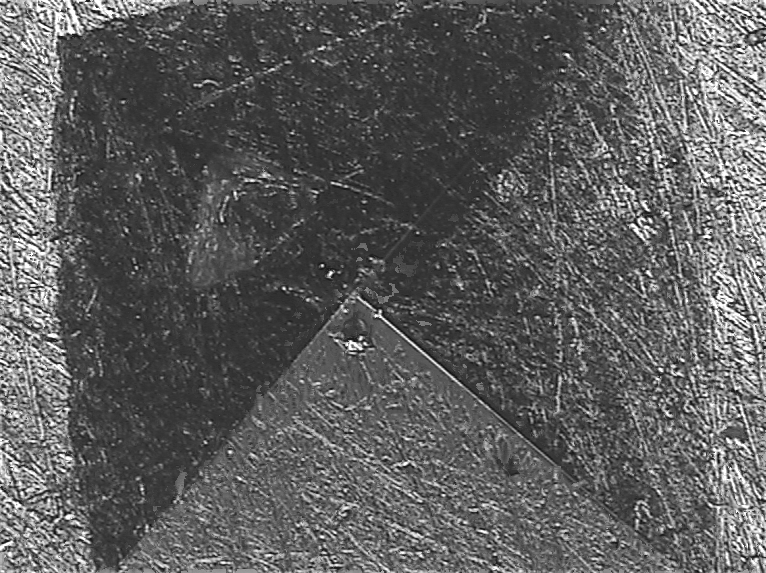
\includegraphics[width=.4\linewidth]{texture_variance_vickers.png}}\hfill
 \subfloat[Altitudes.]{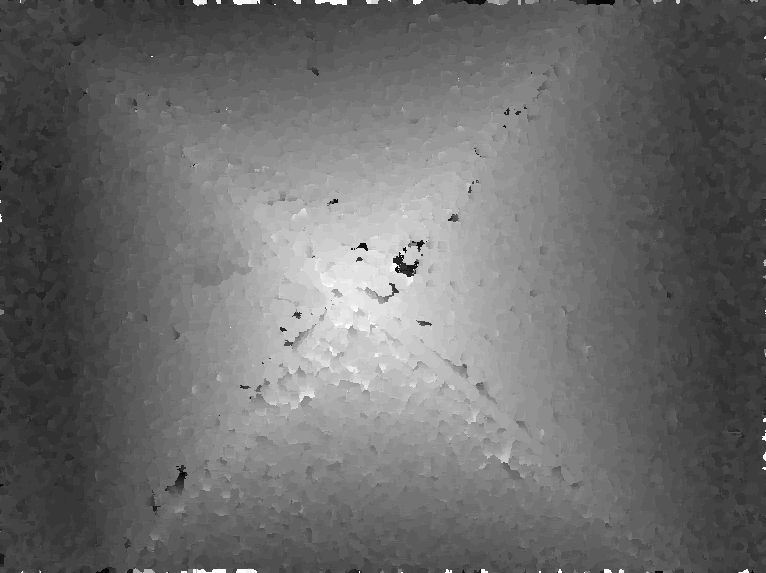
\includegraphics[width=.4\linewidth]{altitude_variance_vickers.png}}

 \subfloat[Texture.]{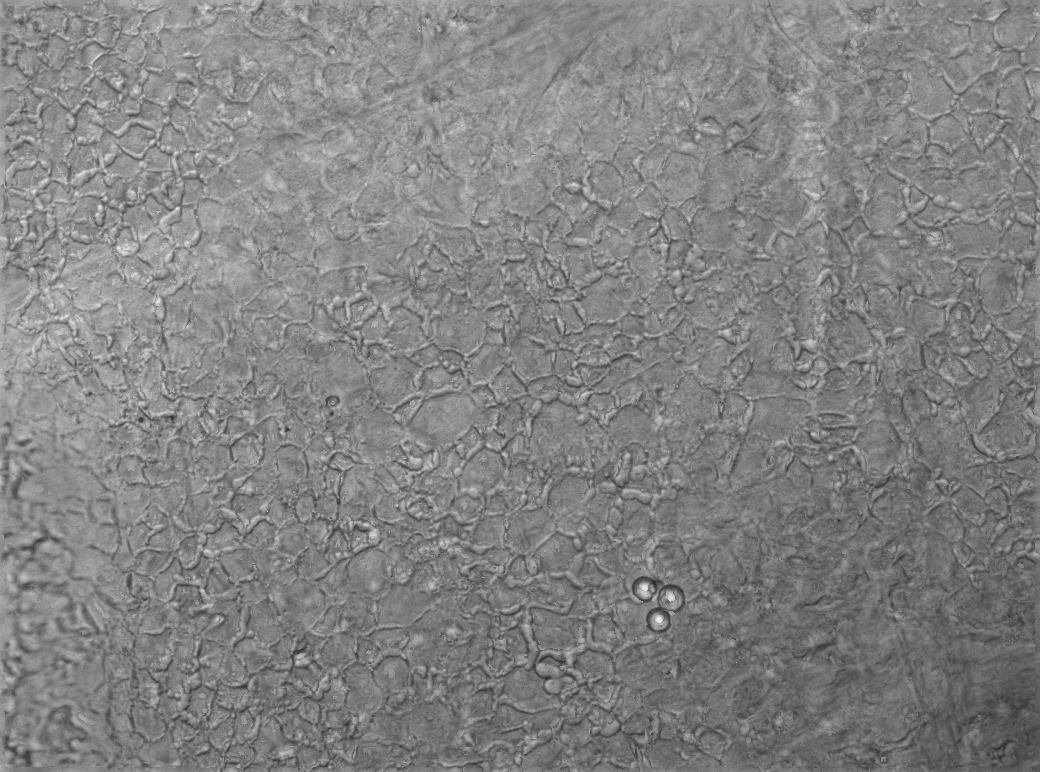
\includegraphics[width=.4\linewidth]{texture_variance_cornee.png}}\hfill
 \subfloat[Altitudes.]{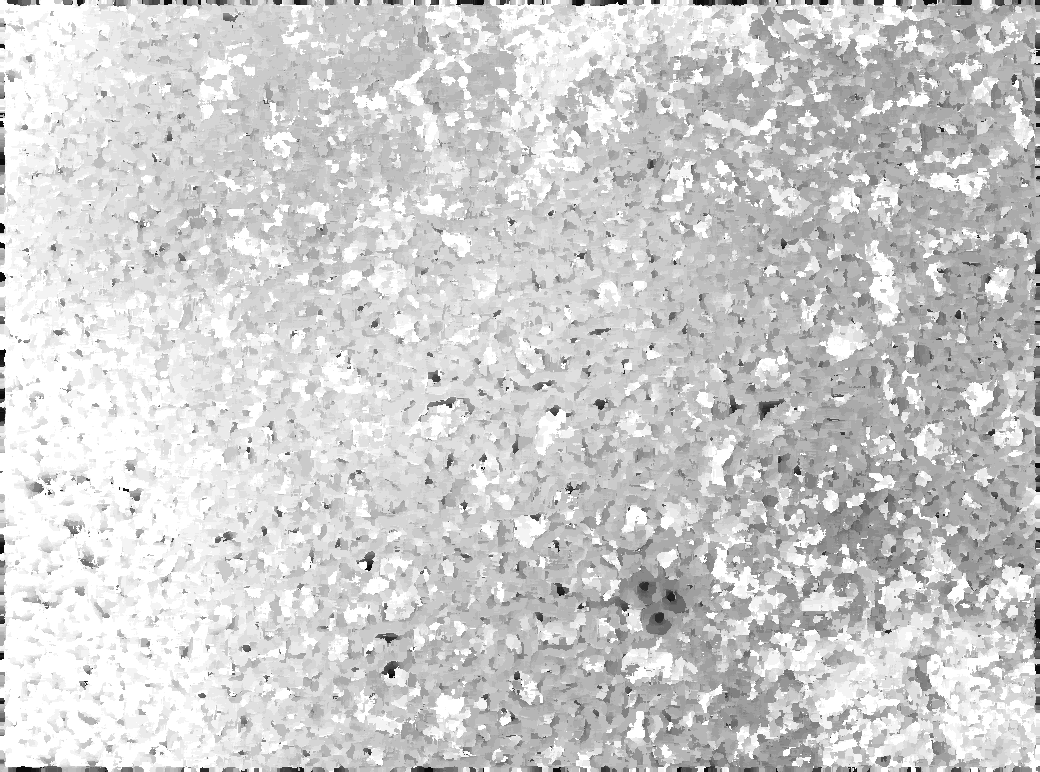
\includegraphics[width=.4\linewidth]{altitude_variance_cornee.png}}
 
 \caption{Texture and altitude reconstruction with the variance method.}
 \label{fig:sff:matlab:variance}
 
\end{figure}

\begin{matlab}
function V=variance(A, N)
% A: single image
% N: size of the window
h = ones(N);

moyenne = (1/N^2) * conv2(A, h, 'same');
D2=(A-moyenne).^2;
% variance
V = conv2(D2, h, 'same');
end
\end{matlab}

\subsection{Tenengrad}
The tenengrad method is base on a Sobel filter, see Fig.\ref{fig:sff:matlab:tenengrad}.

\begin{matlab}
function T=tenengrad(A, ~)
% A: single image
   Sx = fspecial('sobel');
   Gx = imfilter(double(A), Sx, 'replicate', 'conv');
   Gy = imfilter(double(A), Sx', 'replicate', 'conv');
   T = Gx.^2 + Gy.^2;
end
\end{matlab}

\begin{figure}[htbp]
 \centering
 \subfloat[Texture.]{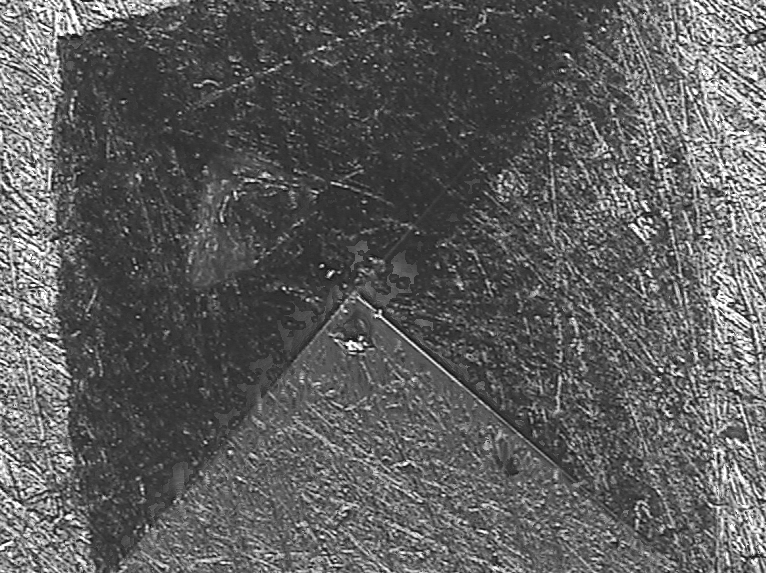
\includegraphics[width=.4\linewidth]{texture_tenengrad_vickers.png}}\hfill
 \subfloat[Altitudes.]{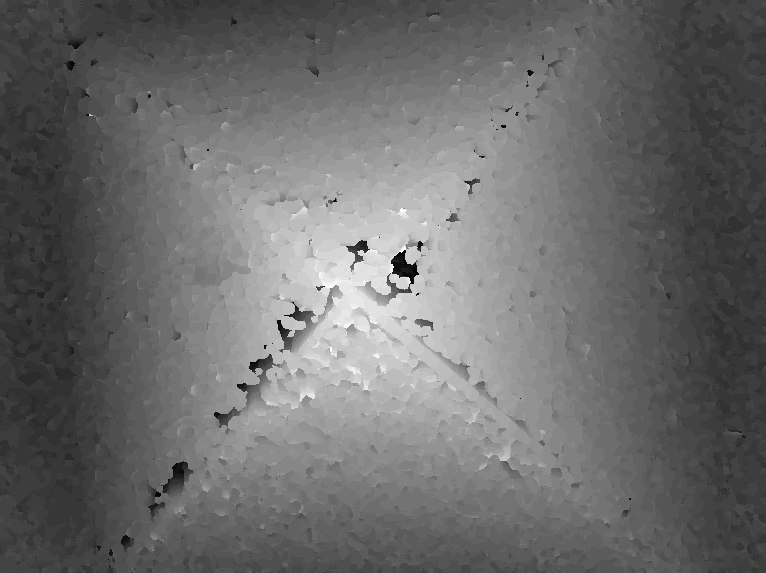
\includegraphics[width=.4\linewidth]{altitude_tenengrad_vickers.png}}

 \subfloat[Texture.]{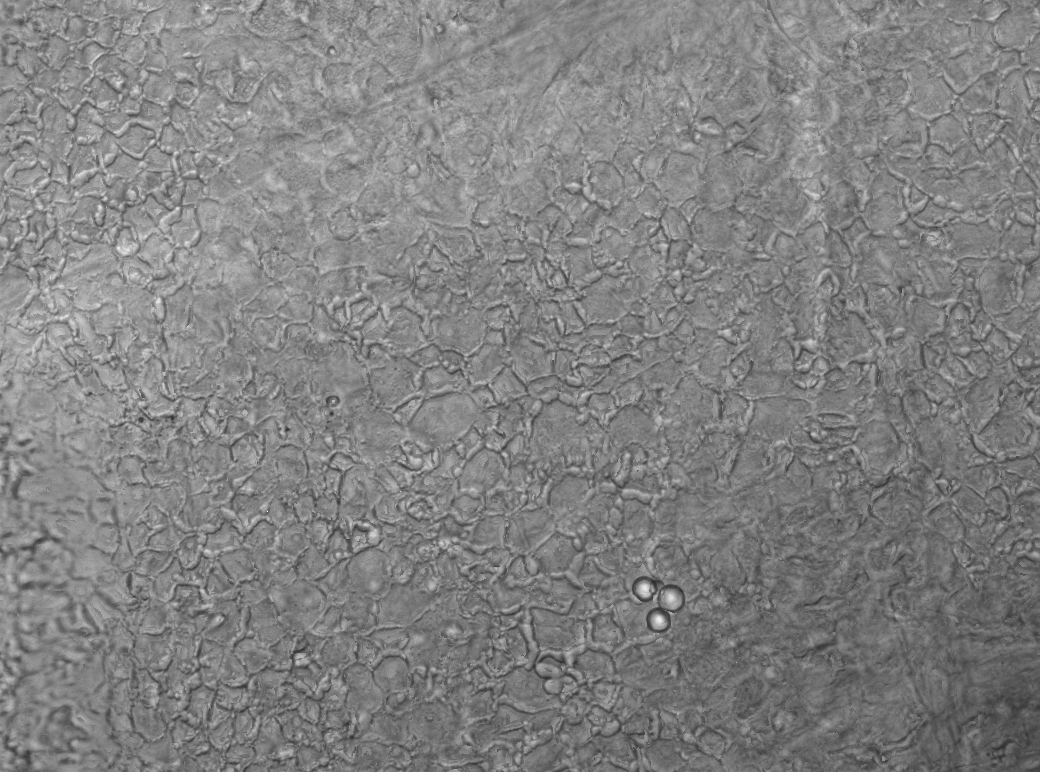
\includegraphics[width=.4\linewidth]{texture_tenengrad_cornee.png}}\hfill
 \subfloat[Altitudes.]{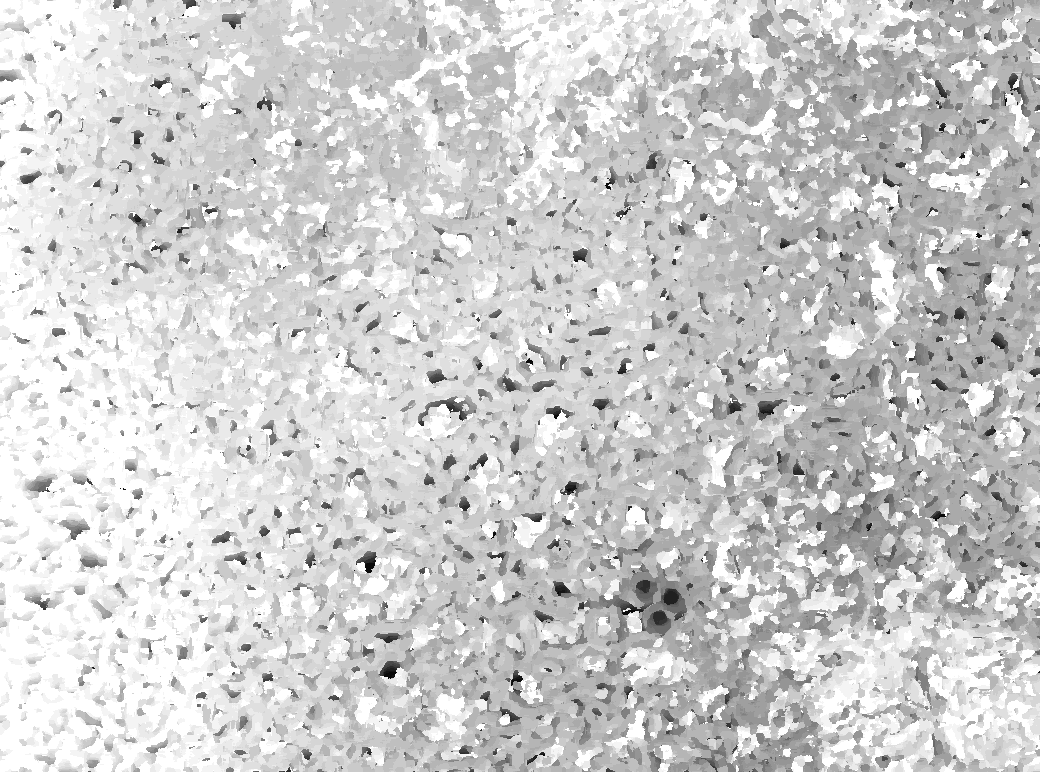
\includegraphics[width=.4\linewidth]{altitude_tenengrad_cornee.png}}
 
 \caption{Texture and altitude reconstruction with the SML method.}
 \label{fig:sff:matlab:tenengrad}
 
\end{figure}

\subsection{Variance of Tenengrad}
The variance of Tenengrad is an improvement of the Tenengrad method, see Fig.\ref{fig:sff:matlab:variancetenengrad}.

\begin{matlab}
function vt=varianceTenengrad(A, N)
   h1 = [1 2 1; 0 0 0; -1 -2 -1];
   h2 = h1';
   ML = sqrt(conv2(A, h1, 'same').^2 + conv2(A, h2, 'same').^2);
        
   vt=variance(ML, N); % variance function previously defined
end

\end{matlab}


\begin{figure}[htbp]
 \centering
 \subfloat[Texture.]{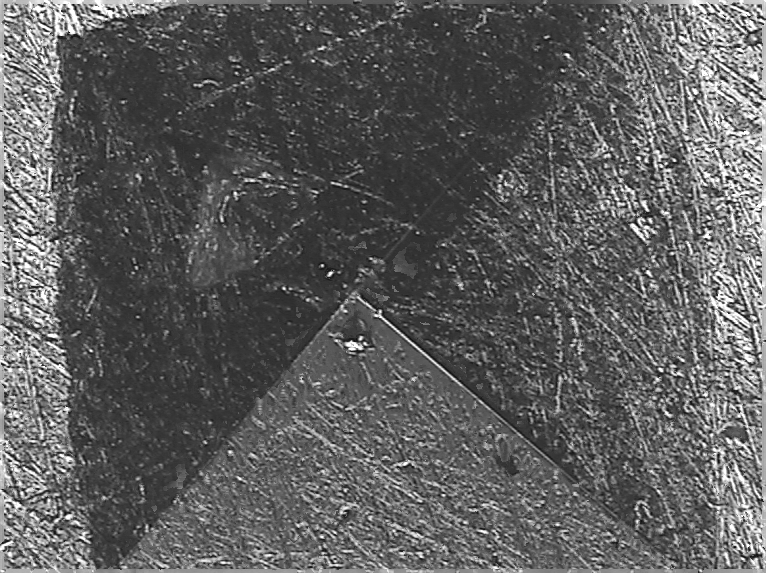
\includegraphics[width=.4\linewidth]{texture_varianceTenengrad_vickers.png}}\hfill
 \subfloat[Altitudes.]{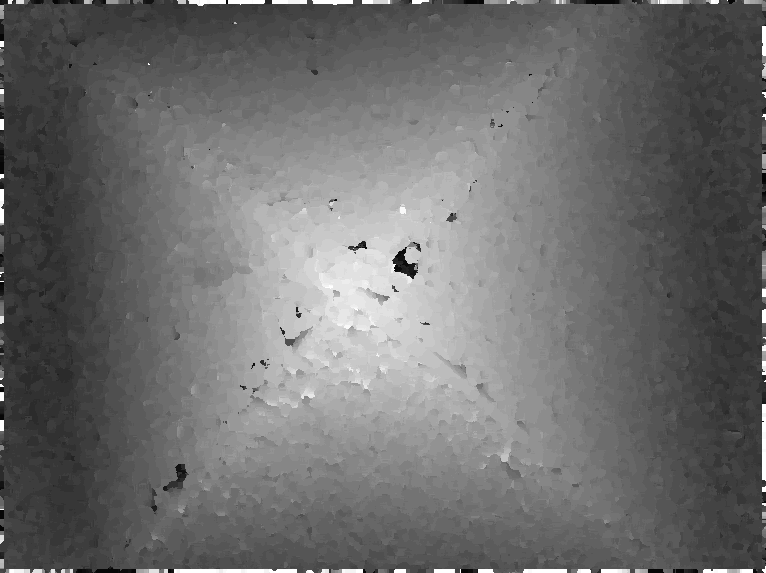
\includegraphics[width=.4\linewidth]{altitude_varianceTenengrad_vickers.png}}

 \subfloat[Texture.]{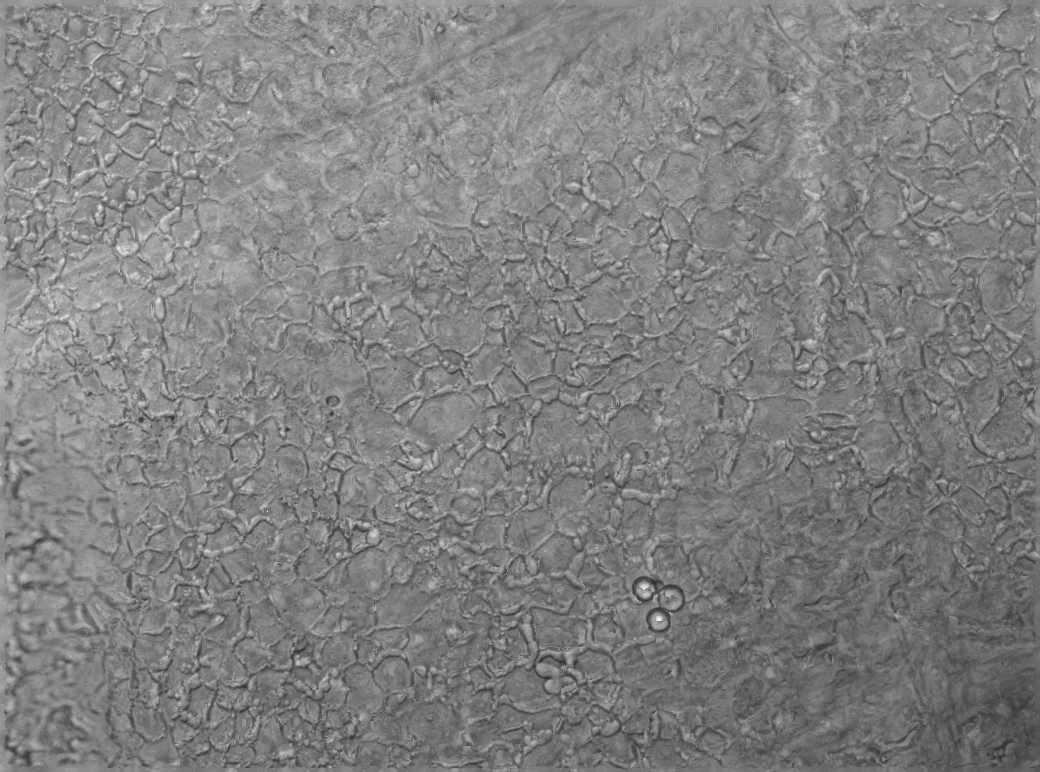
\includegraphics[width=.4\linewidth]{texture_varianceTenengrad_cornee.png}}\hfill
 \subfloat[Altitudes.]{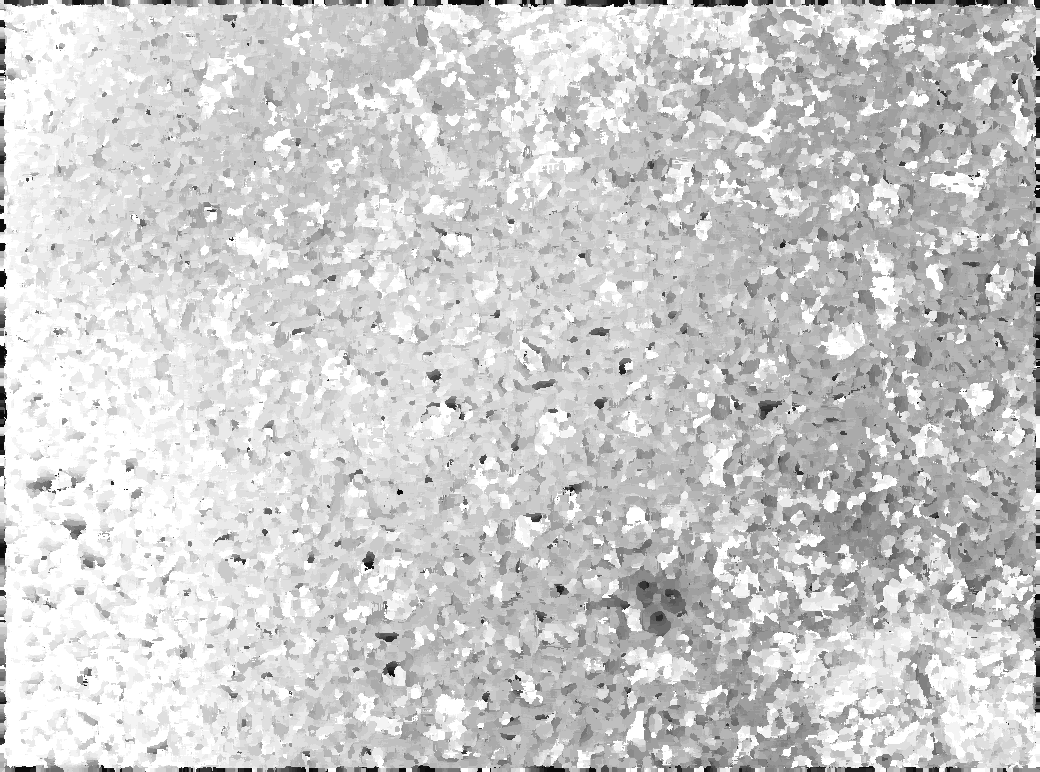
\includegraphics[width=.4\linewidth]{altitude_varianceTenengrad_cornee.png}}
 
 \caption{Texture and altitude reconstruction with the variance of Tenengrad method.}
 \label{fig:sff:matlab:variancetenengrad}
 
\end{figure}